\documentclass[../dissertation.tex]{subfiles}
 
\begin{document}

\section{Experiment 1}

\subsection{Methods}
\subsubsection{Participants}
\begin{wraptable}[8]{r}{0.35\linewidth}
\vspace{-15pt}
\caption{Group sizes for each order}
\vspace{-10pt}
\begin{center}
\begin{tabularx}{0.3\textwidth}{ Y|Y|Y } 
 \hline 
 Effect & Group & \textit{N} \\ 
 \hline
 \multirow{2}{*}{1} & 1 & 40 \\ 
 & 2 & 38 \\ 
 \hline
  \multirow{2}{*}{2} & 3 & 39 \\ 
 & 4 & 39 \\
 \hline 
  \multirow{2}{*}{3} & 5 & 36\\ 
 & 6 & 37 \\ 
 \hline
\end{tabularx}
\end{center}
\label{exp1Ns}
\end{wraptable} Data was collected from 236 undergraduate psychology students at the University of Connecticut (161 Female, 67 Male, mean age = 18.94). Data for the category learning task was lost for 7 subjects due to technical errors. Thus, the final sample size was 229. Each subject was placed into one of six groups. Each group completed two blocks of the category learning task in a specific order. For more details, see Table \ref{exp1order}. Unequal group sizes result from lost data due to technical errors.

\subsubsection{Category Learning Task}
	This task measures learning of dense and sparse categories and is based off of a paradigm from previous research \citep{Kloos2008}. Participants learn novel categories of items in four possible conditions in a 2 x 2 design. The first manipulation is learning type (supervised vs. unsupervised). In \textit{supervised} learning, participants learn the categories by being instructed on the relevant features (e.g., “All friendly aliens have big noses.”). Images of the relevant features are provided along with the descriptions. In \textit{unsupervised} learning, participants learn the categories by viewing sixteen instances of the category. \par
	The second manipulation is category type (sparse vs. dense). Category type is measured by statistical density, which ranges from zero (where all features vary freely) to one (where all features co-occur perfectly). It is based on a comparison between within- and between-category entropy \citep{Sloutsky2010}. All categories in this experiment have seven dimensions. The \textit{sparse} categories cohere on a single dimension, while the other dimensions vary freely (density = .25). In contrast, the \textit{dense} categories cohere on six of the seven dimensions (density = .75). The seventh dimension is allowed to vary freely. For more details on how density was calculated, see Appendix A. Stimuli for each of the four blocks are different. See Fig. \ref{sloutskymanip} for examples of the experimental manipulations. \par
\begin{figure}[htp]
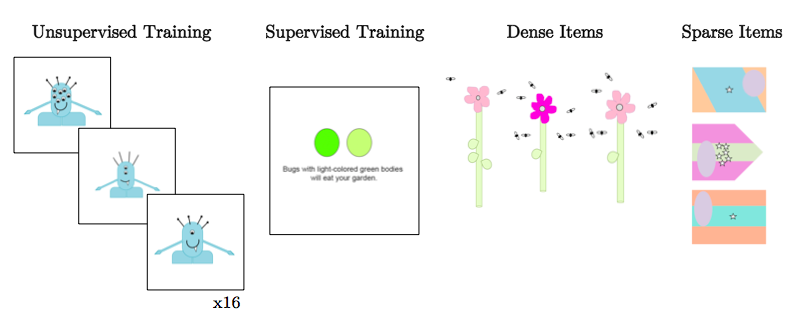
\includegraphics[width=\textwidth]{manipulations}
\caption[Example stimuli for category learning task]{Examples of learning type and category type manipulations for category learning experiment.}
\vspace{-10pt}
\label{sloutskymanip}
\end{figure}
	This task is within-subjects. Based on the group they were placed into, participants completed two of the four possible learning-category type combinations. In this experiment, I tested three main order effects. First, I tested order effects for the matching conditions (unsupervised-dense and supervised-sparse).The second order effect used unsupervised-dense and supervised-dense blocks. Finally, the third order effect tested the same sparse stimuli, testing unsupervised-dense and supervised-sparse blocks. This design led to six possible order groups that each participant could be placed into. See Table \ref{exp1order} for a summary. 
	\begin{wraptable}[11]{r}{0.6\linewidth}
\caption{Block orders for statistical density task}
%\vspace{-10pt}
\begin{center}
\begin{tabular}{ c|c|c|c } 
 \hline 
 Effect & Group & Block 1 & Block 2 \\ 
 \hline
 \multirow{2}{*}{1} & 1 & Unsupervised-dense & Supervised-sparse \\ 
 & 2 & Supervised-sparse & Unsupervised-dense \\ 
 \hline
  \multirow{2}{*}{2} & 3 & Unsupervised-dense & Supervised-dense \\ 
 & 4 & Supervised-dense & Unsupervised-dense \\
 \hline 
  \multirow{2}{*}{3} & 5 & Unsupervised-sparse & Supervised-sparse \\ 
 & 6 & Supervised-sparse & Unsupervised-sparse \\ 
 \hline
\end{tabular}
\end{center}
\vspace{-20pt}
\label{exp1order}
\end{wraptable} \par
 In each block, participants were introduced to the task through a short cover story. They were told to learn which items go with a certain property (e.g., which aliens are friendly). Crucially, no labels were attached to the categories (e.g., some aliens are Ziblets). Then, participants completed a training block (either supervised or unsupervised). After training, participants completed 40 test trials (16 target, 16 distractor, 8 catch), following the design of \citet{Kloos2008} . In each trial, participants saw a single item and used the keyboard to indicate whether the item matched the category they had just learned (e.g., if the alien is friendly). Catch items looked significantly different than both the target and competing categories, so participants should have always rejected them as members of the learned category. This experiment was presented using PsychoPy v.1.84.2 \citep{Peirce2007}. \par

\subsubsection{Behavioral Measures}
	I used multiple assessments to test participants' language ability. The choice of assessments was based on the epiSLI criteria for language impairment \citep{Tomblin1996}, which includes comprehension, expression, vocabulary, grammar, and narrative. I adapted these requirements from a kindergarten population to a college-aged population. The epiSLI criteria have been shown to be robust for diagnosis of specific language impairment (SLI). In addition, other studies of language impairment more broadly have adapted a similar multidimensional approach to measuring language ability, sometimes including measures of phonological skills \citep{Catts2006}. Thus, using assessments that the many domains of language outlined in epiSLI criteria will allow me to get a fuller picture of individual differences in language ability. See Table \ref{slitable} for a summary of the assessments and which domains of the epiSLI criteria they cover. The specific tests used in this experiment are detailed below. \par
	\textbf{Test of word reading efficiency (TOWRE) phonemic decoding subtest.} TOWRE is a test of nonword fluency \citep{Torgesen1992}. This test is a part of the comprehension aspect of epiSLI, since the comprehension measure is reading-based. In the TOWRE, individuals have 45 seconds to read as many nonwords as possible. The nonwords become longer and more difficult as the list goes on. \par
	\textbf{Woodcock Johnson-III word attack (WA) subtest.} This task measures nonword decoding ability \citep{Woodcock2001}. Like the TOWRE, it is helpful for measuring the comprehension aspect of epiSLI. However, while the TOWRE measures word fluency, this task measures decoding accuracy. Participants read a list of nonwords out loud at their own pace. \par
	\textbf{Computerized reading comprehension.} This test covers the comprehension and narrative aspects of epiSLI. This computerized reading comprehension test is based on the Kaufman Test of Educational Achievement (KTEA) reading comprehension subtest \citep{Kaufman2004}. To create this test, I copied the passages and questions contained in the KTEA reading comprehension subtest into E-Prime \citep{schneider2002prime} for presentation on a computer. I created multiple choice answers for the KTEA questions that did not already have them. In this task, participants read short expository and narrative texts and answered multiple-choice comprehension questions about them. Some questions are literal, while others require participants to make an inference. Because this task is a modified version of the KTEA, I use raw scores in analysis rather than standardized scores based on the KTEA norms. \par
	\textbf{Nelson-Denny vocabulary subtest.} The Nelson-Denny vocabulary sub-test is a written assessment of vocabulary \citep{Brown1981}. This test covers the vocabulary aspect of epiSLI. This test has been used in multiple studies of college-aged adults and provides sufficient variability for individual difference investigations in this population \citetext{e.g., \citealt{Boudewyn2015}; \citealt{Stafura2014}}. In this test, participants are asked to choose the word closest to a target vocabulary word. \par
	\textbf{Clinical Evaluation of Language Fundamentals recalling sentences subtest.} I will use the recalling sentences subtest from the Clinical Evaluation of Language Fundamentals \citetext{CELF; \citealt{Semel2006}; \citealt{Stafura2014}}. This test covers the grammar and expression aspects of epiSLI. In this subtest, participants hear sentences and are asked to repeat them. Scoring is based on how many errors the participant makes in their repetition.  \par
	Finally, I used Set II of Raven's Advanced Matrices to measure nonverbal IQ \citep{Raven1998}. In this task, participants see a grid containing eight images and an empty space. The images are arranged in the grid according to some rule or rules. Participants must choose one of eight additional images that fits in the empty space.

\begin{table}[H]
\caption{Assessments of language and their corresponding epiSLI domains.}
\vspace{-10pt}
\begin{center}
\begin{tabular}{ c|c } 
 \hline 
 Test & epiSLI Criteria \\ 
 \hline
 TOWRE & \multirow{2}{*}{Comprehension (decoding aspect)}\\ 
 WA & \\ 
 Computerized Reading Comprehension & Comprehension, narrative \\
 ND Vocab & Vocabulary \\ 
 CELF RS & Grammar, expression \\ 
 \hline
\end{tabular}
\end{center}
\label{slitable}
\end{table}


\subsection{Procedure}
	Each participant completed the category learning task as well as all of the behavioral measures. TOWRE, WA, and CELF were audio-recorded to allow for offline scoring. To allow multiple subjects to be run in a single timeslot, some participants received tasks they could complete on their own (category learning, ND, Computerized reading comprehension, Raven's) first while others completed tasks with the experimenter first (WA, CELF, TOWRE). All together, the seven tasks took approximately one hour.
	
\subsection{Results}
	For all analyses shown below, accuracy was converted to \textit{d'} values \citep{macmillan2004} using the R package \textbf{neuropsychology} \citep{neuropsych}. Correction for extreme values was done following \citep{Hautus1995}. Following prior research, all blocks where 5 or fewer catch items were correctly rejected were dropped from analysis. This resulted in 22 total missing blocks (out of 458 total), including both blocks from a single subject in group 5. \par
	
\subsubsection{Order Effect 1: Matching Conditions}
\begin{wrapfigure}{r}{0.5\textwidth}
\vspace{-10pt}
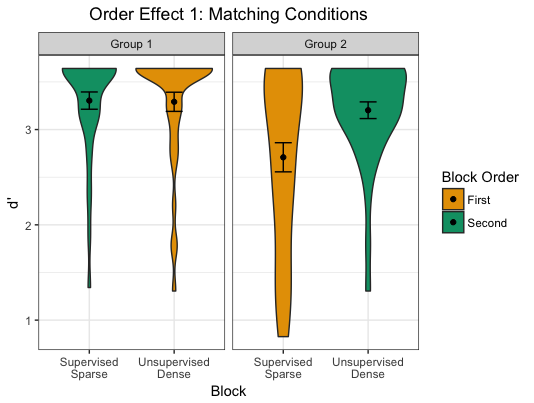
\includegraphics[width=0.5\textwidth]{oe1.png}
\caption[Accuracy plot for order effect 1]{Accuracy (d') for each block completed by each group for the first order effect. Colors indicate which block was encountered first by each group. Points indicate means with error bars reflecting standard error. Shaded portions represent the distribution of accuracy values; wider portions indicate more subjects with that accuracy value.}
\label{oe1}
\vspace{-10pt}
\end{wrapfigure}	
	The first analysis investigated order effects for blocks in which the learning type (supervised vs. unsupervised) and category type (sparse vs. dense) both engaged the same category learning system (hypothesis testing vs. associative). Participants completed supervised-sparse and unsupervised-dense blocks. \par
	I used linear mixed-effects models to examine the effects of block and order on accuracy at test. The relationship between accuracy and block/order showed significant variance in intercepts across participants \textit{SD} = 0.26. Adding block and order as fixed effects significantly increased model fit, $\chi^{2}(2)$ = 13.04,  \textit{p} = 0.001. Adding the interaction between block and order further improved model fit $\chi^{2}(1)$ = 6.05,  \textit{p} = 0.014. Thus, the final model had fixed effects of block, order, and the interaction between block and order as well as random intercepts for subject. \par
	The final model revealed three significant effects. First, there was not a significant main effect of block, \textit{b} = -0.52, \textit{SE} = 0.32, \textit{t}(74) = -1.60, \textit{p} = 0.12. This model also showed a significant main effect of order, \textit{b} = -0.59, \textit{SE} = 0.16, \textit{t}(141) = -3.76, \textit{p} = 0.0002. Finally, there was a significant interaction between block and order, \textit{b} = 0.51, \textit{SE} = 0.20, \textit{t}(72) = 2.48, \textit{p} = 0.016. This interaction was broken down by conducting two separate models for each of the orders (unsupervised-dense first and supervised-sparse first). These analyses showed that when the associative system was engaged first (unsupervised-dense first), there was no significant main effect of block, \textit{b} = -0.0064, \textit{SE} = 0.11, \textit{t}(34) = -0.057, \textit{p} = 0.95. When the hypothesis testing system was used first (supervised-sparse first), there is a significant effect of block, \textit{b} = 0.50, \textit{SE} = 0.17, \textit{t}(37) = 2.92, \textit{p} = 0.0059. Inspection of means shows that when participants complete the supervised-sparse block first, performance on the supervised-sparse block is lower than in the unsupervised-dense block (see Figure \ref{oe1}).

\subsubsection{Order Effect 2: Dense Stimuli}
\begin{wrapfigure}{R}{0.5\textwidth}
\vspace{-10pt}
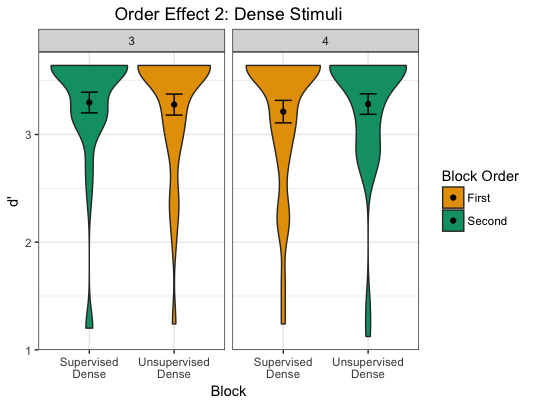
\includegraphics[width=0.5\textwidth]{oe2.png}
\caption[Accuracy plot for order effect 2]{Accuracy (d') for each block completed by each group for the second order effect.}
\label{oe2}
\vspace{-10pt}
\end{wrapfigure}	
	The second order effect analysis compared groups 3 and 4. All participants learned only dense categories, with the order of learning types differing between groups. Again, I used linear-mixed effects models to investigate the effects of block and order on accuracy at test. The variance in intercepts across participants had a standard deviation of 0.62. Adding the fixed effects to the model did not significantly improve fit $\chi^{2}(2)$ = 0.24,  \textit{p} = 0.89. Inspection of coefficients confirmed this finding. Block was not a significant predictor of accuracy, \textit{b} = 0.03, \textit{SE} = 0.10, \textit{t}(145) = 0.27, \textit{p} = 0.79. Similarly, order was not a significant predictor of accuracy, \textit{b} = -0.04, \textit{SE} = 0.10, \textit{t}(145) = -0.11, \textit{p} = 0.68. Thus, accuracy at test on dense categories was similar regardless of training type or block order (see Figure \ref{oe2}).

\subsubsection{Order Effect 3: Sparse Stimuli}
\begin{wrapfigure}{L}{0.5\textwidth}
\vspace{-10pt}
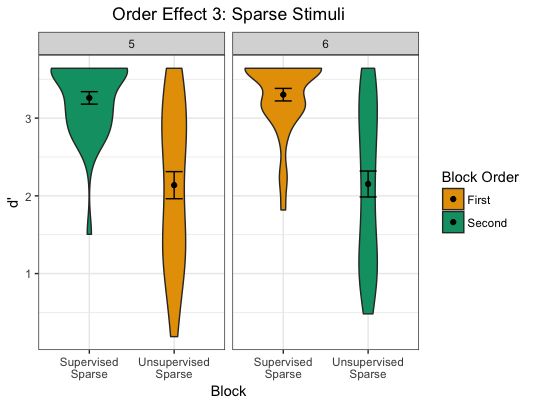
\includegraphics[width=0.5\textwidth]{oe3.png}
\caption[Accuracy plot for order effect 3]{Accuracy (d') for each block completed by each group for the third order effect.}
\label{oe3}
\vspace{-10pt}
\end{wrapfigure}	
	The third order effect investigated differences in learning sparse categories based on learning type order, using data from groups 5 and 6. I used the same type of linear mixed-effect models as the prior two order effects. Random intercepts for subject had a standard deviation of 0.11. Adding block as a fixed effect significantly increased model fit, $\chi^{2}(1)$ = 59.44,  \textit{p} \textless 0.00001. Adding order to this model  did not further improve model fit $\chi^{2}(1)$ = 0.05,  \textit{p} = 0.82. Thus, the final model had a fixed effects of block as well as random intercepts for subject, but no fixed effect of order or interaction between block and order. This model revealed a significant main effect of block, \textit{b} = -1.14, \textit{SE} = 0.13, \textit{t}(72) = -8.91, \textit{p} \textless  0.00001. Inspection of means showed that participants exhibited better performance in supervised-sparse blocks than in unsupervised-dense blocks (see Figure \ref{oe3}).
	
\subsubsection{Exploratory Order Analyses}
An interesting feature of this experimental design is that both manipulations (learning type and category type) push individuals towards a certain category learning system. Supervised and sparse blocks encourage use of the hypothesis-testing system, while unsupervised and dense blocks evoke the associative system. Thus, mismatch blocks (i.e., unsupervised-sparse and supervised-dense) have conflicting information on which category learning system to use and thus likely are less effective at evoking that system. To investigate this possibility, I completed some exploratory analyses.\par
	First, I compared unsupervised-dense blocks completed by groups 2 and 4. Group 2 completed a supervised-sparse (matching, hypothesis-testing) block before their supervised-dense block, while group 4 completed a supervised-dense (mismatch, hypothesis-testing) block before their unsupervised-dense block. If matching blocks more strongly evoke the category learning system and the hypothesized order effect (where activating the hypothesis-testing system first interferes with later use of the associative system) holds, then performance in group 2 on the unsupervised-dense block should be worse than performance in group 4 on the same block. A two-sample \textit{t}-test indicated that this hypothesis did not hold -- the two groups had equivalent performance (\textit{t}(73) = -0.62, \textit{p} = 0.54).\par
	I extended this analysis by doing the sample thing for groups 1 and 5, who both completed the supervised-sparse block second. Group 1 completed an unsupervised-dense (match, associative) block before their supervised-sparse block and group 4 completed an unsupervised-sparse (mismatch, associative) block first. Again, a two-sample \textit{t}-test indicated that the two groups had equivalent performance (\textit{t}(69) = 0.36, \textit{p} = 0.71). \par
	As an additional check, I looked at two more comparisons. First, I compared the unsupervised-dense blocks for the two groups who completed it first, group 1 and group 3. There should be no difference between these groups on this block, since it was the first block each group encountered.  A two-sample \textit{t}-test confirmed this hypothesis (\textit{t}(70) = 0.097, \textit{p} = 0.92). I then checked the same thing for the supervised-sparse blocks within groups 2 and 6. Interestingly, these two groups were found to be different (\textit{t}(54) = -3.43, \textit{p} = 0.001).
\subsection{Discussion}
\subsubsection{Order Effects}
	The primary analyses looked at three different order effect. Each effect compared different ways to engage the hypothesis testing system before the associative system and vice versa. The first order effect used category learning blocks whose learning type and category type matched (i.e., supervised-sparse/hypothesis-testing, unsupervised-dense/associative). A significant interaction was found between block and order. Individuals who completed the unsupervised-dense/associative block first showed similar performance on both blocks. However, participants who completed the supervised-sparse/hypothesis-testing blocks first showed reduced performance in the supervised-sparse/hypothesis-testing block, with considerable recovery by the time they got to the unsupervised-dense/associative blocks. This result may be spurious, however, because the individuals in group 2 showed atypically low accuracy on their first block (supervised-sparse/hypothesis-testing), as compared to participants in group 6 that received the same block first and exhibited higher performance. \par
	Overall, few order effects were found in accuracy. Most performance was close to ceiling. The main effect of block found in the third order analysis indicated that the unsupervised-sparse block may be more difficult overall. This is consistent with prior between-subjects research showing the worst performance in the unsupervised-sparse condition \citep{Kloos2008}.
\subsubsection{Individual Differences}
\end{document}

